\documentclass[twoside]{book}

% Packages required by doxygen
\usepackage{fixltx2e}
\usepackage{calc}
\usepackage{doxygen}
\usepackage[export]{adjustbox} % also loads graphicx
\usepackage{graphicx}
\usepackage[utf8]{inputenc}
\usepackage{makeidx}
\usepackage{multicol}
\usepackage{multirow}
\PassOptionsToPackage{warn}{textcomp}
\usepackage{textcomp}
\usepackage[nointegrals]{wasysym}
\usepackage[table]{xcolor}

% Font selection
\usepackage[T1]{fontenc}
\usepackage[scaled=.90]{helvet}
\usepackage{courier}
\usepackage{amssymb}
\usepackage{sectsty}
\renewcommand{\familydefault}{\sfdefault}
\allsectionsfont{%
  \fontseries{bc}\selectfont%
  \color{darkgray}%
}
\renewcommand{\DoxyLabelFont}{%
  \fontseries{bc}\selectfont%
  \color{darkgray}%
}
\newcommand{\+}{\discretionary{\mbox{\scriptsize$\hookleftarrow$}}{}{}}

% Page & text layout
\usepackage{geometry}
\geometry{%
  a4paper,%
  top=2.5cm,%
  bottom=2.5cm,%
  left=2.5cm,%
  right=2.5cm%
}
\tolerance=750
\hfuzz=15pt
\hbadness=750
\setlength{\emergencystretch}{15pt}
\setlength{\parindent}{0cm}
\setlength{\parskip}{3ex plus 2ex minus 2ex}
\makeatletter
\renewcommand{\paragraph}{%
  \@startsection{paragraph}{4}{0ex}{-1.0ex}{1.0ex}{%
    \normalfont\normalsize\bfseries\SS@parafont%
  }%
}
\renewcommand{\subparagraph}{%
  \@startsection{subparagraph}{5}{0ex}{-1.0ex}{1.0ex}{%
    \normalfont\normalsize\bfseries\SS@subparafont%
  }%
}
\makeatother

% Headers & footers
\usepackage{fancyhdr}
\pagestyle{fancyplain}
\fancyhead[LE]{\fancyplain{}{\bfseries\thepage}}
\fancyhead[CE]{\fancyplain{}{}}
\fancyhead[RE]{\fancyplain{}{\bfseries\leftmark}}
\fancyhead[LO]{\fancyplain{}{\bfseries\rightmark}}
\fancyhead[CO]{\fancyplain{}{}}
\fancyhead[RO]{\fancyplain{}{\bfseries\thepage}}
\fancyfoot[LE]{\fancyplain{}{}}
\fancyfoot[CE]{\fancyplain{}{}}
\fancyfoot[RE]{\fancyplain{}{\bfseries\scriptsize Generated by Doxygen }}
\fancyfoot[LO]{\fancyplain{}{\bfseries\scriptsize Generated by Doxygen }}
\fancyfoot[CO]{\fancyplain{}{}}
\fancyfoot[RO]{\fancyplain{}{}}
\renewcommand{\footrulewidth}{0.4pt}
\renewcommand{\chaptermark}[1]{%
  \markboth{#1}{}%
}
\renewcommand{\sectionmark}[1]{%
  \markright{\thesection\ #1}%
}

% Indices & bibliography
\usepackage{natbib}
\usepackage[titles]{tocloft}
\setcounter{tocdepth}{3}
\setcounter{secnumdepth}{5}
\makeindex

% Hyperlinks (required, but should be loaded last)
\usepackage{ifpdf}
\ifpdf
  \usepackage[pdftex,pagebackref=true]{hyperref}
\else
  \usepackage[ps2pdf,pagebackref=true]{hyperref}
\fi
\hypersetup{%
  colorlinks=true,%
  linkcolor=blue,%
  citecolor=blue,%
  unicode%
}

% Custom commands
\newcommand{\clearemptydoublepage}{%
  \newpage{\pagestyle{empty}\cleardoublepage}%
}

\usepackage{caption}
\captionsetup{labelsep=space,justification=centering,font={bf},singlelinecheck=off,skip=4pt,position=top}

%===== C O N T E N T S =====

\begin{document}

% Titlepage & ToC
\hypersetup{pageanchor=false,
             bookmarksnumbered=true,
             pdfencoding=unicode
            }
\pagenumbering{alph}
\begin{titlepage}
\vspace*{7cm}
\begin{center}%
{\Large R\+O\+CR \\[1ex]\large 1.\+0 }\\
\vspace*{1cm}
{\large Generated by Doxygen 1.8.13}\\
\end{center}
\end{titlepage}
\clearemptydoublepage
\pagenumbering{roman}
\tableofcontents
\clearemptydoublepage
\pagenumbering{arabic}
\hypersetup{pageanchor=true}

%--- Begin generated contents ---
\chapter{File Index}
\section{File List}
Here is a list of all documented files with brief descriptions\+:\begin{DoxyCompactList}
\item\contentsline{section}{/home/markose/catkin\+\_\+ws/src/project\+\_\+rocr\+\_\+bot/rocr/src/\hyperlink{teleop_8cpp}{teleop.\+cpp} \\*Teleop to move the robot and to open and close arms }{\pageref{teleop_8cpp}}{}
\end{DoxyCompactList}

\chapter{File Documentation}
\hypertarget{teleop_8cpp}{}\section{/home/markose/catkin\+\_\+ws/src/project\+\_\+rocr\+\_\+bot/rocr/src/teleop.cpp File Reference}
\label{teleop_8cpp}\index{/home/markose/catkin\+\_\+ws/src/project\+\_\+rocr\+\_\+bot/rocr/src/teleop.\+cpp@{/home/markose/catkin\+\_\+ws/src/project\+\_\+rocr\+\_\+bot/rocr/src/teleop.\+cpp}}


Teleop to move the robot and to open and close arms.  


{\ttfamily \#include $<$ros/ros.\+h$>$}\newline
{\ttfamily \#include $<$geometry\+\_\+msgs/\+Twist.\+h$>$}\newline
{\ttfamily \#include $<$std\+\_\+msgs/\+Float64.\+h$>$}\newline
{\ttfamily \#include $<$stdio.\+h$>$}\newline
{\ttfamily \#include $<$unistd.\+h$>$}\newline
{\ttfamily \#include $<$termios.\+h$>$}\newline
{\ttfamily \#include $<$map$>$}\newline
{\ttfamily \#include $<$algorithm$>$}\newline
Include dependency graph for teleop.\+cpp\+:
\nopagebreak
\begin{figure}[H]
\begin{center}
\leavevmode
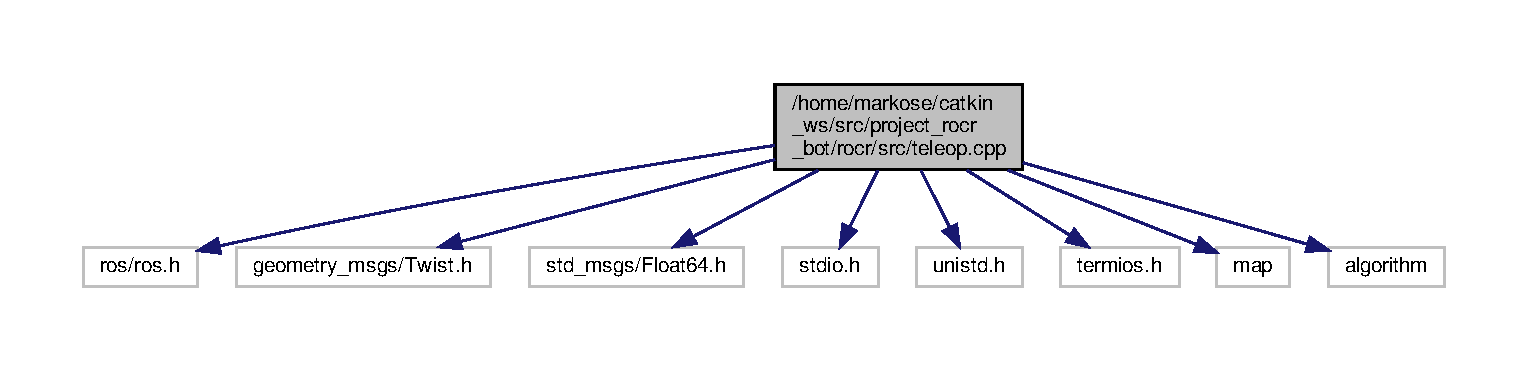
\includegraphics[width=350pt]{teleop_8cpp__incl}
\end{center}
\end{figure}
\subsection*{Functions}
\begin{DoxyCompactItemize}
\item 
float \hyperlink{teleop_8cpp_a0c412d48ccdce40e00c45eae6a90f28a}{speed} (0.\+5)
\begin{DoxyCompactList}\small\item\em Init Variables. \end{DoxyCompactList}\item 
\mbox{\Hypertarget{teleop_8cpp_addb83adac8170dcb113acaf93aeccf82}\label{teleop_8cpp_addb83adac8170dcb113acaf93aeccf82}} 
float {\bfseries turn} (1.\+0)
\item 
\mbox{\Hypertarget{teleop_8cpp_a58456ccdd2b0d0e7ebb96c0a2ec7ec6f}\label{teleop_8cpp_a58456ccdd2b0d0e7ebb96c0a2ec7ec6f}} 
float {\bfseries x} (0)
\item 
\mbox{\Hypertarget{teleop_8cpp_a2795aa30f97a85f1d013e24f6292a51e}\label{teleop_8cpp_a2795aa30f97a85f1d013e24f6292a51e}} 
float {\bfseries y} (0)
\item 
\mbox{\Hypertarget{teleop_8cpp_aec5d3cf4e6cb26ab7be21502b97087c9}\label{teleop_8cpp_aec5d3cf4e6cb26ab7be21502b97087c9}} 
float {\bfseries z} (0)
\item 
\mbox{\Hypertarget{teleop_8cpp_ad5ac4dec8b4343953b42a1e86edb874e}\label{teleop_8cpp_ad5ac4dec8b4343953b42a1e86edb874e}} 
float {\bfseries th} (0)
\item 
\mbox{\Hypertarget{teleop_8cpp_a84133027073931c36d3cf6fec12d5ff3}\label{teleop_8cpp_a84133027073931c36d3cf6fec12d5ff3}} 
float {\bfseries arm\+\_\+movement} (0)
\item 
\mbox{\Hypertarget{teleop_8cpp_a707311ac31b1d2e00c843eae201a6536}\label{teleop_8cpp_a707311ac31b1d2e00c843eae201a6536}} 
char {\bfseries key} (\textquotesingle{} \textquotesingle{})
\item 
int \hyperlink{teleop_8cpp_af5978fab9fa6dd4ced1c3a8ab1251f7b}{getch} (void)
\begin{DoxyCompactList}\small\item\em For non-\/blocking keyboard inputs. \end{DoxyCompactList}\item 
int \hyperlink{teleop_8cpp_a3c04138a5bfe5d72780bb7e82a18e627}{main} (int argc, char $\ast$$\ast$argv)
\end{DoxyCompactItemize}
\subsection*{Variables}
\begin{DoxyCompactItemize}
\item 
std\+::map$<$ char, std\+::vector$<$ float $>$ $>$ {\bfseries move\+Bindings}
\item 
std\+::map$<$ char, std\+::vector$<$ float $>$ $>$ {\bfseries speed\+Bindings}
\item 
std\+::map$<$ char, std\+::vector$<$ float $>$ $>$ {\bfseries arm\+Bindings}
\item 
\mbox{\Hypertarget{teleop_8cpp_a2c3cb87d009c003069b9a90f020f8a9f}\label{teleop_8cpp_a2c3cb87d009c003069b9a90f020f8a9f}} 
const char $\ast$ {\bfseries msg}
\end{DoxyCompactItemize}


\subsection{Detailed Description}
Teleop to move the robot and to open and close arms. 

2021 Markose Jacob, Yash Mandar Kulkarni, Vivek Sood

\begin{DoxyAuthor}{Author}
Markose Jacob, Yash Mandar Kulkarni, Vivek Sood 
\end{DoxyAuthor}
\begin{DoxyDate}{Date}
12/12/2021
\end{DoxyDate}
Original open source code taken from git clone \href{https://github.com/methylDragon/teleop_twist_keyboard_cpp.git}{\tt https\+://github.\+com/methyl\+Dragon/teleop\+\_\+twist\+\_\+keyboard\+\_\+cpp.\+git}\hypertarget{teleop_8cpp_LICENSE}{}\subsection{L\+I\+C\+E\+N\+SE}\label{teleop_8cpp_LICENSE}
M\+IT License Copyright (c) 2021 Markose Jacob, Yash Mandar Kulkarni, Vivek Sood Permission is hereby granted, free of charge, to any person obtaining a copy of this software and associated documentation files (the \char`\"{}\+Software\char`\"{}), to deal in the Software without restriction, including without limitation the rights to use, copy, modify, merge, publish, distribute, sublicense, and/or sell copies of the Software, and to permit persons to whom the Software is furnished to do so, subject to the following conditions\+:

The above copyright notice and this permission notice shall be included in all copies or substantial portions of the Software.

T\+HE S\+O\+F\+T\+W\+A\+RE IS P\+R\+O\+V\+I\+D\+ED \char`\"{}\+A\+S I\+S\char`\"{}, W\+I\+T\+H\+O\+UT W\+A\+R\+R\+A\+N\+TY OF A\+NY K\+I\+ND, E\+X\+P\+R\+E\+SS OR I\+M\+P\+L\+I\+ED, I\+N\+C\+L\+U\+D\+I\+NG B\+UT N\+OT L\+I\+M\+I\+T\+ED TO T\+HE W\+A\+R\+R\+A\+N\+T\+I\+ES OF M\+E\+R\+C\+H\+A\+N\+T\+A\+B\+I\+L\+I\+TY, F\+I\+T\+N\+E\+SS F\+OR A P\+A\+R\+T\+I\+C\+U\+L\+AR P\+U\+R\+P\+O\+SE A\+ND N\+O\+N\+I\+N\+F\+R\+I\+N\+G\+E\+M\+E\+NT. IN NO E\+V\+E\+NT S\+H\+A\+LL T\+HE A\+U\+T\+H\+O\+RS OR C\+O\+P\+Y\+R\+I\+G\+HT H\+O\+L\+D\+E\+RS BE L\+I\+A\+B\+LE F\+OR A\+NY C\+L\+A\+IM, D\+A\+M\+A\+G\+ES OR O\+T\+H\+ER L\+I\+A\+B\+I\+L\+I\+TY, W\+H\+E\+T\+H\+ER IN AN A\+C\+T\+I\+ON OF C\+O\+N\+T\+R\+A\+CT, T\+O\+RT OR O\+T\+H\+E\+R\+W\+I\+SE, A\+R\+I\+S\+I\+NG F\+R\+OM, O\+UT OF OR IN C\+O\+N\+N\+E\+C\+T\+I\+ON W\+I\+TH T\+HE S\+O\+F\+T\+W\+A\+RE OR T\+HE U\+SE OR O\+T\+H\+ER D\+E\+A\+L\+I\+N\+GS IN T\+HE S\+O\+F\+T\+W\+A\+RE.\hypertarget{teleop_8cpp_DESCRIPTION}{}\subsection{D\+E\+S\+C\+R\+I\+P\+T\+I\+ON}\label{teleop_8cpp_DESCRIPTION}
Teleop for R\+O\+CR bot 

\subsection{Function Documentation}
\mbox{\Hypertarget{teleop_8cpp_af5978fab9fa6dd4ced1c3a8ab1251f7b}\label{teleop_8cpp_af5978fab9fa6dd4ced1c3a8ab1251f7b}} 
\index{teleop.\+cpp@{teleop.\+cpp}!getch@{getch}}
\index{getch@{getch}!teleop.\+cpp@{teleop.\+cpp}}
\subsubsection{\texorpdfstring{getch()}{getch()}}
{\footnotesize\ttfamily int getch (\begin{DoxyParamCaption}\item[{void}]{ }\end{DoxyParamCaption})}



For non-\/blocking keyboard inputs. 

\begin{DoxyReturn}{Returns}
int 
\end{DoxyReturn}
\mbox{\Hypertarget{teleop_8cpp_a3c04138a5bfe5d72780bb7e82a18e627}\label{teleop_8cpp_a3c04138a5bfe5d72780bb7e82a18e627}} 
\index{teleop.\+cpp@{teleop.\+cpp}!main@{main}}
\index{main@{main}!teleop.\+cpp@{teleop.\+cpp}}
\subsubsection{\texorpdfstring{main()}{main()}}
{\footnotesize\ttfamily int main (\begin{DoxyParamCaption}\item[{int}]{argc,  }\item[{char $\ast$$\ast$}]{argv }\end{DoxyParamCaption})}

Init R\+OS node


\begin{DoxyParams}{Parameters}
{\em nh} & R\+OS Node\+Handle\\
\hline
\end{DoxyParams}
Publisher for cmd\+\_\+vel topic to rotate wheels and move arms 
\begin{DoxyParams}{Parameters}
{\em pub} & cmd\+\_\+vel publisher \\
\hline
{\em pub\+\_\+right\+\_\+arm} & cmd\+\_\+vel publisher \\
\hline
{\em pub\+\_\+left\+\_\+arm} & cmd\+\_\+vel publisher\\
\hline
\end{DoxyParams}
Creating Twist and Float messages for wheels and arms respectivly 
\begin{DoxyParams}{Parameters}
{\em twist} & for wheels \\
\hline
{\em arm\+\_\+control} & for left arm \\
\hline
{\em arm\+\_\+control\+\_\+2} & for right arm\\
\hline
\end{DoxyParams}
While loop which ends only when the program is terminated. Keep taking in put from the user and compares it with the key map Appropriate action is taken based on user choice\mbox{\Hypertarget{teleop_8cpp_a0c412d48ccdce40e00c45eae6a90f28a}\label{teleop_8cpp_a0c412d48ccdce40e00c45eae6a90f28a}} 
\index{teleop.\+cpp@{teleop.\+cpp}!speed@{speed}}
\index{speed@{speed}!teleop.\+cpp@{teleop.\+cpp}}
\subsubsection{\texorpdfstring{speed()}{speed()}}
{\footnotesize\ttfamily float speed (\begin{DoxyParamCaption}\item[{0.}]{5 }\end{DoxyParamCaption})}



Init Variables. 


\begin{DoxyParams}{Parameters}
{\em speed} & Linear velocity (m/s) \\
\hline
{\em turn} & Angular velocity (rad/s) \\
\hline
{\em x} & Forward direction \\
\hline
{\em y} & backward direction \\
\hline
{\em z} & neutral direction \\
\hline
{\em th} & angle direction \\
\hline
{\em arm\+\_\+movements} & Arm Movement \\
\hline
{\em key} & To read the key entered \\
\hline
\end{DoxyParams}


\subsection{Variable Documentation}
\mbox{\Hypertarget{teleop_8cpp_a6d6f9af1f8240c66439917581344ed3b}\label{teleop_8cpp_a6d6f9af1f8240c66439917581344ed3b}} 
\index{teleop.\+cpp@{teleop.\+cpp}!arm\+Bindings@{arm\+Bindings}}
\index{arm\+Bindings@{arm\+Bindings}!teleop.\+cpp@{teleop.\+cpp}}
\subsubsection{\texorpdfstring{arm\+Bindings}{armBindings}}
{\footnotesize\ttfamily std\+::map$<$char, std\+::vector$<$float$>$ $>$ arm\+Bindings}

{\bfseries Initial value\+:}
\begin{DoxyCode}
\{
  \{\textcolor{charliteral}{'1'}, \{0.0, 0\}\},
  \{\textcolor{charliteral}{'2'}, \{-0.1, 0\}\}
\}
\end{DoxyCode}
\mbox{\Hypertarget{teleop_8cpp_a91023ea7582580513b585f7b4c15f7d8}\label{teleop_8cpp_a91023ea7582580513b585f7b4c15f7d8}} 
\index{teleop.\+cpp@{teleop.\+cpp}!move\+Bindings@{move\+Bindings}}
\index{move\+Bindings@{move\+Bindings}!teleop.\+cpp@{teleop.\+cpp}}
\subsubsection{\texorpdfstring{move\+Bindings}{moveBindings}}
{\footnotesize\ttfamily std\+::map$<$char, std\+::vector$<$float$>$ $>$ move\+Bindings}

{\bfseries Initial value\+:}
\begin{DoxyCode}
\{
  \{\textcolor{charliteral}{'i'}, \{1, 0, 0, 0\}\},
  \{\textcolor{charliteral}{'o'}, \{1, 0, 0, -1\}\},
  \{\textcolor{charliteral}{'j'}, \{0, 0, 0, 1\}\},
  \{\textcolor{charliteral}{'l'}, \{0, 0, 0, -1\}\},
  \{\textcolor{charliteral}{'u'}, \{1, 0, 0, 1\}\},
  \{\textcolor{charliteral}{','}, \{-1, 0, 0, 0\}\},
  \{\textcolor{charliteral}{'.'}, \{-1, 0, 0, 1\}\},
  \{\textcolor{charliteral}{'m'}, \{-1, 0, 0, -1\}\},
  \{\textcolor{charliteral}{'O'}, \{1, -1, 0, 0\}\},
  \{\textcolor{charliteral}{'I'}, \{1, 0, 0, 0\}\},
  \{\textcolor{charliteral}{'J'}, \{0, 1, 0, 0\}\},
  \{\textcolor{charliteral}{'L'}, \{0, -1, 0, 0\}\},
  \{\textcolor{charliteral}{'U'}, \{1, 1, 0, 0\}\},
  \{\textcolor{charliteral}{'<'}, \{-1, 0, 0, 0\}\},
  \{\textcolor{charliteral}{'>'}, \{-1, -1, 0, 0\}\},
  \{\textcolor{charliteral}{'M'}, \{-1, 1, 0, 0\}\},
  \{\textcolor{charliteral}{'t'}, \{0, 0, 1, 0\}\},
  \{\textcolor{charliteral}{'b'}, \{0, 0, -1, 0\}\},
  \{\textcolor{charliteral}{'k'}, \{0, 0, 0, 0\}\},
  \{\textcolor{charliteral}{'K'}, \{0, 0, 0, 0\}\}
\}
\end{DoxyCode}
\mbox{\Hypertarget{teleop_8cpp_a942d4f1c3e151d6f264d0868766b08b0}\label{teleop_8cpp_a942d4f1c3e151d6f264d0868766b08b0}} 
\index{teleop.\+cpp@{teleop.\+cpp}!speed\+Bindings@{speed\+Bindings}}
\index{speed\+Bindings@{speed\+Bindings}!teleop.\+cpp@{teleop.\+cpp}}
\subsubsection{\texorpdfstring{speed\+Bindings}{speedBindings}}
{\footnotesize\ttfamily std\+::map$<$char, std\+::vector$<$float$>$ $>$ speed\+Bindings}

{\bfseries Initial value\+:}
\begin{DoxyCode}
\{
  \{\textcolor{charliteral}{'q'}, \{1.1, 1.1\}\},
  \{\textcolor{charliteral}{'z'}, \{0.9, 0.9\}\},
  \{\textcolor{charliteral}{'w'}, \{1.1, 1\}\},
  \{\textcolor{charliteral}{'x'}, \{0.9, 1\}\},
  \{\textcolor{charliteral}{'e'}, \{1, 1.1\}\},
  \{\textcolor{charliteral}{'c'}, \{1, 0.9\}\}
\}
\end{DoxyCode}

%--- End generated contents ---

% Index
\backmatter
\newpage
\phantomsection
\clearemptydoublepage
\addcontentsline{toc}{chapter}{Index}
\printindex

\end{document}
